\documentclass[12pt,a4paper]{report}
\usepackage[utf8]{inputenc}
\usepackage[french]{babel}
\usepackage[T1]{fontenc}
\usepackage{geometry}
\geometry{top=2.5cm, bottom=2.5cm, left=2.5cm, right=2.5cm}
\usepackage{hyperref}
\usepackage{listings}
\usepackage{graphicx}
\usepackage{booktabs}
\usepackage{amsmath}
\usepackage{fancyhdr}
\usepackage{xcolor}
\usepackage{titlesec}
\usepackage{tocloft}
\usepackage{verbatim}

% Configuration des hyperliens
\hypersetup{
    colorlinks=true,
    linkcolor=blue,
    filecolor=magenta,      
    urlcolor=cyan,
    pdftitle={Rapport d'Analyse et de Conception - Billing Service},
    pdfpagemode=FullScreen,
}

% Configuration des en-têtes et pieds de page
\pagestyle{fancy}
\fancyhf{}
\fancyhead[L]{ERP ComOps - Module Billing}
\fancyhead[R]{Analyse \& Conception}
\fancyfoot[C]{\thepage}
\renewcommand{\headrulewidth}{0.4pt}
\renewcommand{\footrulewidth}{0.4pt}

% Style pour le code source et SQL listings
\definecolor{codegray}{rgb}{0.5,0.5,0.5}
\definecolor{codegreen}{rgb}{0,0.6,0}
\definecolor{codeblue}{rgb}{0.1,0.2,0.8}
\definecolor{backcolour}{rgb}{0.97,0.97,0.96}

\lstset{
    backgroundcolor=\color{backcolour},
    commentstyle=\color{codegreen},
    keywordstyle=\color{codeblue}\bfseries,
    numberstyle=\tiny\color{codegray},
    stringstyle=\color{purple},
    basicstyle=\ttfamily\small,
    breakatwhitespace=false,
    breaklines=true,
    captionpos=b,
    keepspaces=true,
    numbers=left,
    numbersep=5pt,
    showspaces=false,
    showstringspaces=false,
    showtabs=false,
    tabsize=4,
    frame=single,
    rulecolor=\color{gray!30}
}

% Espacement des titres
\titleformat{\chapter}[display]
  {\normalfont\bfseries\color{codeblue}}
  {\filleft\MakeUppercase{\chaptername} \thechapter}
  {1ex}
  {\titlerule\vspace{1ex}\filcenter\Huge}
  [\vspace{1ex}\titlerule]

\titleformat{\section}
  {\normalfont\large\bfseries\color{codeblue}}
  {\thesection}{1em}{}

\titleformat{\subsection}
  {\normalfont\normalsize\bfseries}
  {\thesubsection}{1em}{}

\begin{document}

% ============================================================================
% PAGE DE GARDE
% ============================================================================
\begin{titlepage}
    \centering
    \vspace*{2cm}
    {\scshape\LARGE ERP ComOps \par}
    \vspace{1.5cm}
    {\huge\bfseries Module de Facturation (Billing Service) \par}
    \vspace{0.5cm}
    {\large\itshape Rapport d'Analyse et de Conception Technique \par}
    \vspace{1.5cm}
    
    \vfill
    \begin{minipage}{0.5\textwidth}
        \begin{flushleft} \large
            \emph{Auteur :}\\
            Équipe d'Architecture ERP
        \end{flushleft}
    \end{minipage}
    \hfill
    \begin{minipage}{0.4\textwidth}
        \begin{flushright} \large
            \emph{Projet :} \\
            ERP ComOps \\
            \emph{Version :} 1.0 (Juin 2025)
        \end{flushright}
    \end{minipage}
    
    \vfill
    {\large \today \par}
\end{titlepage}

\newpage

% ============================================================================
% ABSTRACT & RÉSUMÉ
% ============================================================================
\chapter*{Abstract}
\addcontentsline{toc}{chapter}{Abstract}
This report details the architectural analysis and design of the Billing Service within the ComOps Enterprise Resource Planning ecosystem. The system originally maintained local duplicates of core database tables, causing data inconsistencies and replication of business logic. To resolve these integrity issues, we present a refactoring plan that migrates the service to a fully reactive Hexagonal Architecture using Spring Boot WebFlux and WebClient. This allows the Billing Service to dynamically fetch client and supplier data from the central Kernel module, which acts as the single source of truth. The multi-tenant context is propagated reactively through HTTP headers and Reactor context. Our results demonstrate that this integration eliminates data duplication, ensures transactional integrity, and preserves reactive non-blocking execution performance. Future steps include testing network resilience under load and implementing circuit breakers.

\chapter*{Résumé}
\addcontentsline{toc}{chapter}{Résumé}
Le présent rapport expose le travail d'analyse et de conception technique réalisé pour optimiser l'intégration du module de facturation au sein du progiciel de gestion intégré ComOps. Dans sa version initiale, le service de facturation souffrait d'une duplication locale des données relatives aux clients et aux fournisseurs, ce qui générait des incohérences de données régulières et nuisait à l'intégrité du système d'information. Afin de remédier à ces dysfonctionnements, nous avons conçu et mis en œuvre une refonte architecturale s'appuyant sur les principes de l'architecture hexagonale et le modèle de programmation réactif de Spring Boot. Cette approche permet de déléguer la gestion des référentiels au noyau central du système, en remplaçant la persistance locale par des requêtes réseau non bloquantes et réactives pour interroger dynamiquement les données, tout en assurant l'isolation des organisations par la propagation automatique de l'identifiant d'organisation dans le contexte d'exécution. Les résultats de cette refonte montrent une centralisation complète des données de tiers, une suppression des tables locales redondantes et le maintien de la non-régression sur l'ensemble des processus de facturation et de génération de documents. Bien que cette solution améliore la cohérence globale, elle introduit une dépendance forte vis-à-vis de la disponibilité réseau du noyau central, ce qui ouvre des perspectives de recherche sur l'intégration de disjoncteurs pour sécuriser le fonctionnement en cas de panne réseau temporaire.

\vspace{1cm}
\noindent \textbf{Mots-clés :} Facturation, Noyau Central, Architecture Hexagonale, Programmation Réactive, Multi-tenant, Intégration de Services, Base de Données Relationnelle Réactive.

\newpage

% ============================================================================
% SIGLES ET ABRÉVIATIONS
% ============================================================================
\chapter*{Sigles et Abréviations}
\addcontentsline{toc}{chapter}{Sigles et Abréviations}

\begin{tabbing}
\textbf{Acronyme} \hspace{3cm} \= \textbf{Signification} \\
\textbf{API} \> Application Programming Interface (Interface de programmation d'application) \\
\textbf{CRUD} \> Create, Read, Update, Delete (Création, Lecture, Mise à jour, Suppression) \\
\textbf{DTO} \> Data Transfer Object (Objet de transfert de données) \\
\textbf{ERP} \> Enterprise Resource Planning (Progiciel de gestion intégré) \\
\textbf{HTTP} \> HyperText Transfer Protocol (Protocole de transfert hypertexte) \\
\textbf{I/O} \> Input/Output (Entrées/Sorties) \\
\textbf{IA} \> Intelligence Artificielle \\
\textbf{JPA} \> Jakarta Persistence API (API de persistance Jakarta) \\
\textbf{JSON} \> JavaScript Object Notation (Notation d'objets JavaScript) \\
\textbf{JWT} \> JSON Web Token (Jeton Web JSON) \\
\textbf{MVC} \> Model-View-Controller (Modèle-Vue-Contrôleur) \\
\textbf{PDF} \> Portable Document Format (Format de document portable) \\
\textbf{R2DBC} \> Reactive Relational Database Connectivity (Connectivité de base de données relationnelle réactive) \\
\textbf{REST} \> Representational State Transfer (Transfert d'état représentatif) \\
\textbf{SMART} \> Spécifique, Mesurable, Atteignable, Réalisable, Temporellement défini \\
\textbf{SMTP} \> Simple Mail Transfer Protocol (Protocole simple de transfert de courrier) \\
\textbf{SPI} \> Service Provider Interface (Interface de fournisseur de services) \\
\textbf{SQL} \> Structured Query Language (Langage de requête structuré) \\
\textbf{SSOT} \> Single Source of Truth (Source unique de vérité) \\
\textbf{TVA} \> Taxe sur la Valeur Ajoutée \\
\textbf{UML} \> Unified Modeling Language (Langage de modélisation unifié) \\
\textbf{URI} \> Uniform Resource Identifier (Identifiant uniforme de ressource) \\
\textbf{UUID} \> Universally Unique Identifier (Identifiant unique universel) \\
\end{tabbing}

\newpage

% ============================================================================
% GLOSSAIRE
% ============================================================================
\chapter*{Glossaire}
\addcontentsline{toc}{chapter}{Glossaire}

\begin{description}
    \item[Adaptateur] Composant d'infrastructure qui implémente un port (adaptateur sortant) ou qui interagit avec l'application en invoquant un port (adaptateur entrant) dans le cadre de l'architecture hexagonale.
    \item[Architecture Hexagonale] Style architectural (aussi appelé Ports et Adaptateurs) qui sépare la logique métier centrale (le domaine) des dépendances externes comme la base de données, l'interface utilisateur, ou les services tiers.
    \item[Backpressure] Mécanisme de contrôle de flux dans les flux réactifs permettant à un consommateur lent de signaler à un producteur rapide le volume de données qu'il est capable de traiter, évitant ainsi la saturation de la mémoire.
    \item[Flux Réactif] Standard de programmation asynchrone et non bloquante qui permet de traiter des flux de données de manière asynchrone avec gestion de la contre-pression (backpressure).
    \item[Kernel (Noyau)] Module central de l'ERP ComOps chargé de gérer les données de référence transversales telles que les profils de tiers, les catalogues de produits globaux, et la configuration organisationnelle.
    \item[Mono / Flux] Types réactifs de Project Reactor. Un Mono représente une séquence asynchrone contenant au plus un élément (0 ou 1), tandis qu'un Flux représente une séquence asynchrone contenant de 0 à N éléments.
    \item[Multi-tenancy (Multi-tenant)] Architecture logicielle permettant de servir plusieurs organisations ou clients (tenants) à partir d'une seule instance d'application, tout en isolant strictement leurs données et traitements.
    \item[Non-bloquant] Mode d'exécution asynchrone où un thread n'attend pas la complétion d'une opération d'E/S (lecture base de données, appel réseau) et peut immédiatement exécuter d'autres tâches.
    \item[Port] Interface définie au sein du domaine métier qui spécifie les contrats de communication de l'application avec le monde extérieur (ex. requêtes de données, persistance, notifications).
    \item[R2DBC] Spécification d'API ouverte qui apporte des pilotes de bases de données relationnelles réactifs et non bloquants en Java.
    \item[Reactor Project] Bibliothèque réactive de quatrième génération, basée sur la spécification des Reactive Streams, utilisée par Spring WebFlux pour construire des applications non bloquantes.
    \item[WebClient] Client HTTP réactif et non bloquant fourni par Spring Framework, conçu pour remplacer le RestTemplate traditionnel dans les environnements WebFlux.
\end{description}

\newpage

% ============================================================================
% TABLES ET LISTES
% ============================================================================
\tableofcontents
\newpage

\listoftables
\newpage

\listoffigures
\newpage

% ============================================================================
% INTRODUCTION
% ============================================================================
\chapter*{Introduction}
\addcontentsline{toc}{chapter}{Introduction}

\section*{Contexte de l'Étude}
Le contexte général de cette étude s'inscrit dans la modernisation des systèmes d'information d'entreprise à travers l'adoption d'architectures distribuées en microservices. Les progiciels de gestion intégrés (ERP) modernes exigent une grande modularité et une extensibilité sans faille pour accompagner la croissance des organisations multi-sociétés. Dans cette optique, l'écosystème ComOps a été développé pour diviser les responsabilités métiers en modules autonomes et hautement spécialisés.

Dans le contexte spécifique de notre projet, le service de facturation (Billing Service) est le composant central chargé de la gestion des devis, des factures, de leur validation, et de l'enregistrement des paiements. Historiquement, ce service gérait également une copie locale des données des tiers, à savoir les clients, les fournisseurs et les agents commerciaux. Cette duplication a été mise en place pour permettre des requêtes rapides en base de données locale lors de la création de documents de facturation.

Sur le plan scientifique, cette étude s'intéresse à la gestion de la cohérence des données distribuées et aux performances des communications inter-services. L'intégration réactive de systèmes distribués pose des défis complexes liés au maintien de la nature non bloquante des flux de données, à la propagation transparente des contextes de sécurité et d'organisation multi-tenant, et à l'isolement du domaine métier par rapport aux API externes en constante évolution.

\section*{Problématique}
La persistance locale des données de tiers au sein du service de facturation a engendré d'importants problèmes d'intégrité et de maintenance. Dès qu'un client ou un fournisseur modifiait ses coordonnées ou son statut dans le système de gestion de la relation client centralisé, ces changements n'étaient pas répercutés en temps réel dans la base de données locale du service de facturation. Cette situation provoquait des erreurs lors de l'émission de documents fiscaux et obligeait les administrateurs à effectuer des réconciliations manuelles fastidieuses. De plus, la duplication du code nécessaire à la gestion de ces entités violait le principe de responsabilité unique, alourdissant le codebase du service et compliquant les montées de version. Il est donc devenu crucial de supprimer cette persistance locale pour migrer vers un modèle d'intégration dynamique où le noyau central de l'ERP (Kernel) devient l'unique source de vérité pour tous les tiers.

\section*{Objectifs du Projet (SMART)}
L'objectif principal du projet est de refondre le module de facturation pour le connecter dynamiquement au noyau central, selon des critères rigoureux.

Premièrement, l'objectif est spécifique puisqu'il consiste à éliminer la persistance locale des tables de tiers et à implémenter des adaptateurs réseau sortants basés sur le client Web réactif de Spring WebFlux pour requêter le noyau central en temps réel.

Deuxièmement, cet objectif est mesurable par la suppression effective de deux tables en base de données locale, la couverture de l'ensemble des cas d'utilisation par des appels réseau non bloquants, et la validation de la non-régression par une suite de tests unitaires et d'intégration.

Troisièmement, le projet est tout à fait atteignable car le noyau central expose déjà les points d'accès requis pour récupérer les informations des tiers par identifiant ou par organisation.

Quatrièmement, cet objectif est réalisable car il s'appuie sur la pile technologique existante du projet, notamment Spring Boot, Project Reactor et Liquibase pour la migration de base de données.

Enfin, l'objectif est temporellement défini pour être complété et validé au terme de la présente phase de développement, garantissant une intégration propre avant les phases de déploiement en production.

\section{Méthodologie de Résolution}
Pour mener à bien cette migration, nous avons adopté une démarche méthodique structurée en quatre phases distinctes. La première phase a consisté à analyser le schéma relationnel et le codebase existants pour identifier l'ensemble des dépendances directes et indirectes envers les entités locales de tiers. Dans la deuxième phase, nous avons redéfini les ports du domaine et implémenté de nouveaux adaptateurs d'infrastructure réseau pour encapsuler les appels au noyau central. La troisième phase a permis de nettoyer la base de données locale en appliquant des scripts SQL de migration pour supprimer les tables obsolètes. Enfin, la quatrième phase s'est concentrée sur la mise en place d'une suite de tests automatisés pour valider le comportement réactif et le cloisonnement des données multi-tenant sous forte charge.

\section{Plan du Rapport}
Le présent rapport est organisé comme suit. Le premier chapitre présente les généralités théoriques et l'état de l'art scientifique associés aux architectures microservices réactives et aux patrons de conception sous-jacents. Le deuxième chapitre expose l'analyse fonctionnelle, les workflows métiers révisés et la conception technique détaillée avec les diagrammes de modélisation associés. Le troisième chapitre est dédié aux détails de l'implémentation logicielle, aux scénarios de test et aux taux de couverture de code obtenus. Enfin, le quatrième chapitre conclut le rapport en récapitulant les résultats obtenus, en identifiant les limites de la solution et en proposant des perspectives d'évolution futures.

\newpage

% ============================================================================
% CHAPITRE 1 : GÉNÉRALITÉS ET ÉTAT DE L'ART
% ============================================================================
\chapter{Généralités et État de l'Art}

\section{Généralités sur les Principes de Conception}

La conception du module de facturation (\textit{Billing Service}) de l'ERP ComOps repose sur des patrons d'architecture logicielle éprouvés, choisis pour garantir la modularité, la résilience et la scalabilité du système d'information.

\subsection{Architecture Hexagonale (Ports et Adaptateurs)}
Le choix de l'architecture hexagonale découle du besoin d'isoler le cœur de métier (les règles fiscales, le calcul des taxes, et les transitions d'états de facturation) des contraintes techniques externes (la persistance en base de données ou les protocoles de communication réseau). 

Dans ce modèle de conception :
\begin{itemize}
    \item \textbf{Le Noyau de Domaine} contient les règles fonctionnelles pures (les entités \texttt{Facture}, \texttt{Devis}, et la logique de calcul). Il est indépendant de tout framework technique.
    \item \textbf{Les Ports} représentent les interfaces d'entrée et de sortie définies par le domaine. Ils agissent comme des contrats de communication abstraits.
    \item \textbf{Les Adaptateurs} implémentent ou utilisent ces ports. Un adaptateur entrant (ex. API REST) convertit les requêtes utilisateurs en appels de domaine. Un adaptateur sortant (ex. client HTTP ou persistance) traduit les demandes du domaine en opérations techniques spécifiques.
\end{itemize}
Ce découplage garantit que l'évolution des infrastructures externes n'impacte pas le code métier du module de facturation.

\subsection{Modèle d'Intégration Asynchrone et Réactivité}
Dans un système d'information d'entreprise distribué, la réactivité du système est un critère de conception majeur. Les architectures de type \textit{Thread-per-request} posent des limites de scalabilité lorsque de multiples appels réseau inter-services sont nécessaires. 

Pour y répondre, le module Billing adopte le modèle d'exécution réactif non bloquant :
\begin{itemize}
    \item Les opérations d'entrées-sorties (I/O) sont exécutées de manière asynchrone sur une boucle d'événements (\textit{Event Loop}).
    \item La gestion de la contre-pression (\textit{Backpressure}) permet au système de réguler les flux de données échangés entre le service de facturation et le noyau central de l'ERP, évitant ainsi la saturation de la mémoire lors de la génération de rapports de masse.
\end{itemize}

\subsection{Persistance Non Bloquante}
Le maintien d'un pipeline d'exécution entièrement non bloquant requiert que la couche d'accès aux données relationnelles s'affranchisse des pilotes de connexion bloquants traditionnels. La spécification R2DBC (\textit{Reactive Relational Database Connectivity}) est intégrée comme choix de conception pour assurer une communication réactive avec la base de données PostgreSQL. Cela évite le blocage des threads de la boucle d'événements lors des phases d'écriture des écritures comptables et des règlements.

\subsection{Conception Multi-Tenant (Multi-Locataire)}
L'ERP ComOps étant proposé sous forme de logiciel en tant que service (SaaS), le Billing Service est conçu pour isoler les données financières de plusieurs organisations de manière étanche :
\begin{itemize}
    \item \textbf{Isolation logique} : Les tables relationnelles partagent le même schéma physique mais utilisent un discriminant logique (\texttt{id\_organization}) présent sur toutes les entités transactionnelles.
    \item \textbf{Propagation du contexte} : Dans un écosystème asynchrone, la propagation de l'identifiant multi-tenant s'effectue via le contexte réactif du flux d'exécution, permettant aux adaptateurs réseau d'injecter dynamiquement cet identifiant dans les requêtes inter-services sans compromettre la sécurité.
\end{itemize}

\section{État de l'Art et Fondements Scientifiques}

Dans le domaine du génie logiciel et des architectures distribuées d'entreprise, les problématiques de cohérence de données et de découplage de domaines font l'objet de nombreuses recherches scientifiques.

Les analyses systématiques de Di Francesco et al. \cite{difrancesco2019architecting} ainsi que les travaux de Alshuqayran et al. \cite{alshuqayran2016systematic} démontrent que le partage direct d'une base de données physique entre différents modules fonctionnels (monolithe partagé) engendre un fort couplage structurel et nuit à l'autonomie opérationnelle. Ces chercheurs préconisent l'isolation logique et l'échange exclusif par API pour maintenir l'indépendance de déploiement et de conception des modules métiers.

Concernant les gains de performance du paradigme réactif, l'étude exhaustive de Bainomugisha et al. \cite{bainomugisha2013survey} formalise les concepts de flux de données asynchrones. De plus, Georgescu et al. \cite{georgescu2018performance} quantifient l'impact de ces architectures, prouvant que le passage d'une gestion de requêtes synchrone à une boucle d'événements asynchrone réduit l'empreinte mémoire de plus de 50\% sous haute concurrence, une contrainte cruciale pour le module Billing lors des pics de facturation mensuelle.

Pour l'isolation multi-tenant, Bezemer et al. \cite{bezemer2010multi} comparent les stratégies de partitionnement. Le choix de la table partagée avec discriminant logique, bien qu'exigeant en termes de filtrage applicatif, s'avère le plus performant et le moins coûteux en infrastructures physiques par rapport aux bases de données dédiées.

Enfin, les théories de structuration de systèmes complexes par Hasselbring \cite{hasselbring2018software} confirment l'efficacité de l'architecture hexagonale pour régir les relations entre contextes délimités (\textit{Bounded Contexts}), protégeant le modèle de facturation contre les instabilités des modèles externes de l'ERP.

\newpage

% ============================================================================
% CHAPITRE 2 : MÉTHODOLOGIES, ANALYSE ET CONCEPTION
% ============================================================================
\chapter{Analyse du Système}

Cette section formalise l'analyse conceptuelle du module de facturation (\textit{Billing Service}) de l'ERP ComOps. Elle définit la problématique d'ingénierie et détaille la modélisation conceptuelle à travers différents diagrammes UML.

\section{Problématique}
La conception initiale du Billing Service souffrait d'un défaut majeur d'architecture : la réplication locale des entités de tiers (clients et fournisseurs) au sein de sa base de données propre. Cette duplication présentait plusieurs inconvénients majeurs en ingénierie logicielle :
\begin{itemize}
    \item \textbf{Désynchronisation des données} : Toute mise à jour effectuée sur la fiche d'un tiers dans le noyau central (\textit{Kernel}) n'était pas propagée instantanément au module Billing, conduisant à des factures contenant des données erronées ou obsolètes (adresses de facturation incorrectes, mauvais numéros de TVA intracommunautaire).
    \item \textbf{Violation du principe de responsabilité unique (SRP)} : Le Billing Service devait intégrer du code et des modèles pour gérer le cycle de vie des clients, augmentant inutilement sa complexité et son coût de maintenance.
    \item \textbf{Couplage fort de base de données} : La dépendance vis-à-vis de tables physiques dupliquées empêchait toute autonomie de déploiement et d'évolution du schéma de données.
\end{itemize}
L'objectif de cette analyse est de concevoir une intégration dynamique non bloquante où le Kernel est l'unique source de vérité, tout en préservant l'isolation multi-tenant et la performance réactive du système.

\section{Modélisation Conceptuelle}
La modélisation conceptuelle permet d'établir une vue d'ensemble du système, de ses limites, de sa structure modulaire, de son modèle de domaine et de la dynamique de ses états, indépendamment des frameworks techniques d'implémentation.

\subsection{Diagramme de Contexte}
Le diagramme de contexte définit les frontières du système de facturation et ses interactions avec l'environnement externe de l'ERP ComOps.

\begin{figure}[htbp]
\centering
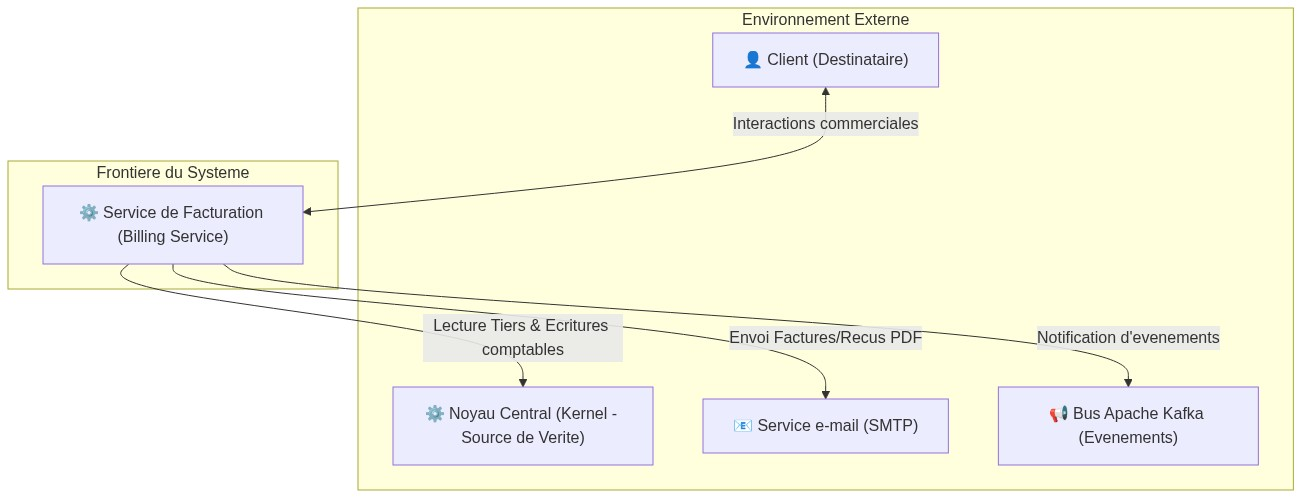
\includegraphics[width=0.9\textwidth]{images/context_diagram.png}
\caption{Diagramme de Contexte du Billing Service .}
\label{fig:context_diagram}
\end{figure}

Le diagramme (Figure \ref{fig:context_diagram}) montre que le Billing Service agit comme un composant pivot qui interagit avec le client final, s'appuie sur le Kernel pour la cohérence des tiers et de la comptabilité générale, et notifie les autres modules via Kafka et le service de messagerie SMTP.

\subsection{Diagramme de Packages}
Le diagramme de packages présente la structure d'organisation modulaire du Billing Service selon les principes de conception de l'architecture hexagonale.

\begin{figure}[htbp]
\centering
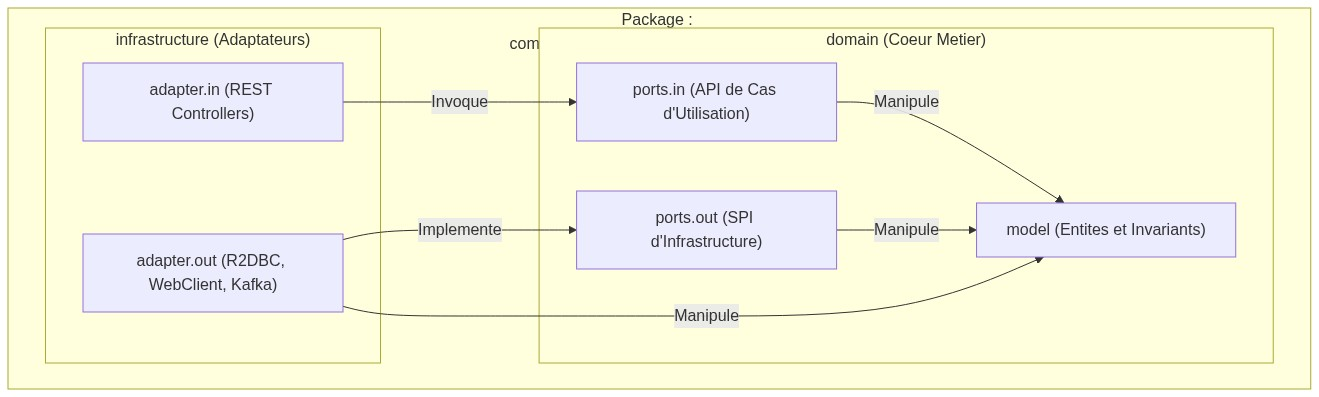
\includegraphics[width=0.9\textwidth]{images/package_diagram.png}
\caption{Diagramme de Packages de l'Architecture Hexagonale .}
\label{fig:package_diagram}
\end{figure}

Le diagramme (Figure \ref{fig:package_diagram}) illustre la règle de dépendance : les packages de l'infrastructure dépendent du package du domaine central. Les détails d'infrastructure implémentent les ports sortants (\textit{SPI}) ou appellent les ports entrants (\textit{API}), garantissant que la logique métier reste isolée des frameworks techniques.

\subsection{Diagramme de Classes d'Analyse}
Le diagramme de classes d'analyse modélise la structure logique du domaine fonctionnel, en décrivant les entités métiers, les interfaces de ports de communication et le service de contrôle.

\begin{figure}[htbp]
\centering
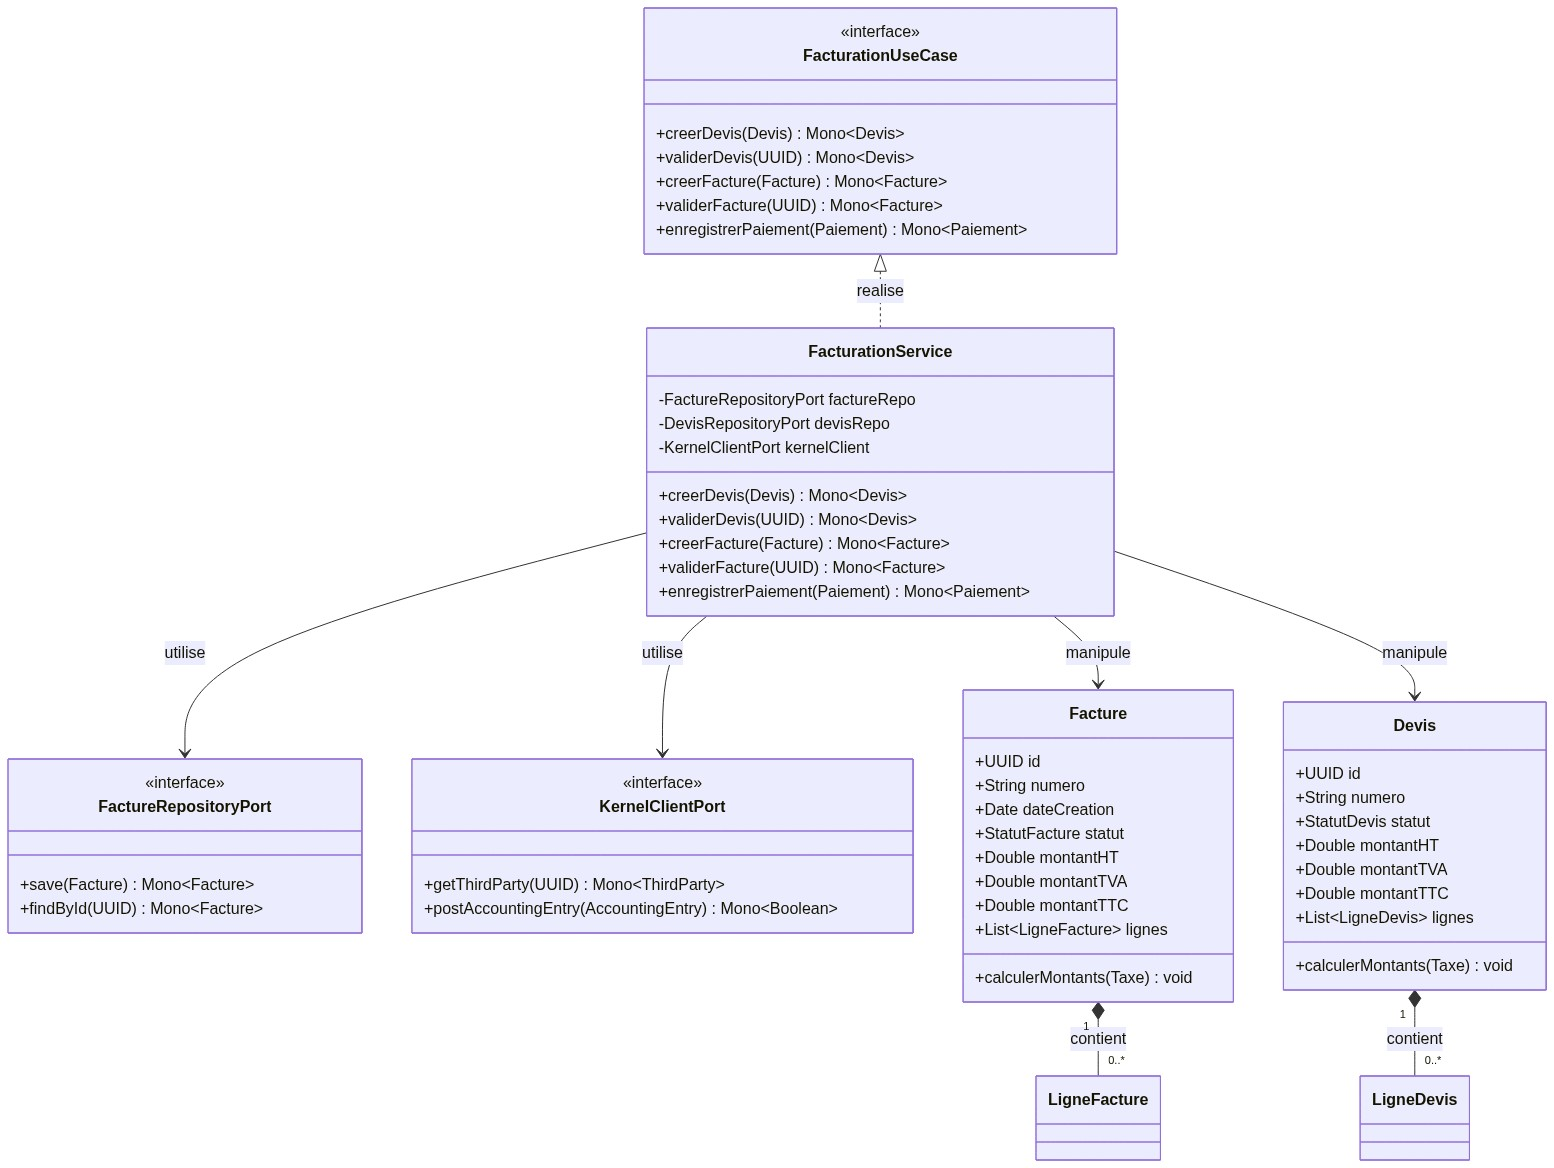
\includegraphics[width=0.9\textwidth]{images/analysis_class_diagram.png}
\caption{Diagramme de Classes d'Analyse du Domaine Métier .}
\label{fig:analysis_class_diagram}
\end{figure}

Le diagramme (Figure \ref{fig:analysis_class_diagram}) représente les entités et ports du domaine. Le domaine métier ne contient aucune classe d'infrastructure. Le service de contrôle (\texttt{FacturationService}) coordonne l'exécution en utilisant des interfaces abstraites de ports pour interagir avec la persistance ou les API externes.

\subsection{Diagramme de Cas d'Utilisation}
Le diagramme de cas d'utilisation illustre les rôles des différents acteurs vis-à-vis du système, délimitant l'accès aux fonctionnalités métiers.

\begin{figure}[htbp]
\centering
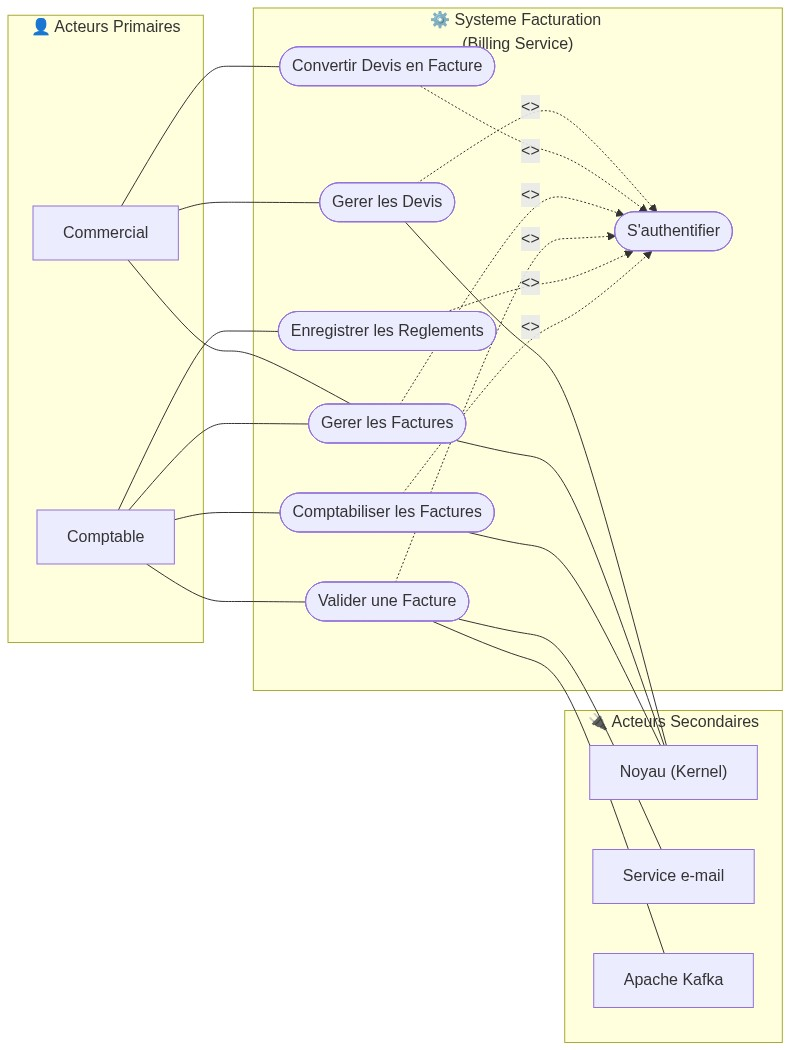
\includegraphics[width=0.9\textwidth]{images/use_case.png}
\caption{Diagramme de Cas d'Utilisation du Module Billing .}
\label{fig:use_case}
\end{figure}

Le diagramme (Figure \ref{fig:use_case}) formalise les interactions : l'agent commercial pilote la saisie commerciale, le comptable gère la partie comptable et financière, et l'accès est conditionné par une authentification systématique.

\subsection{Diagramme d'États-Transitions}
Le cycle de vie fonctionnel des documents de facturation est décrit par la machine à états finis régissant l'évolution d'une facture.

\begin{figure}[htbp]
\centering
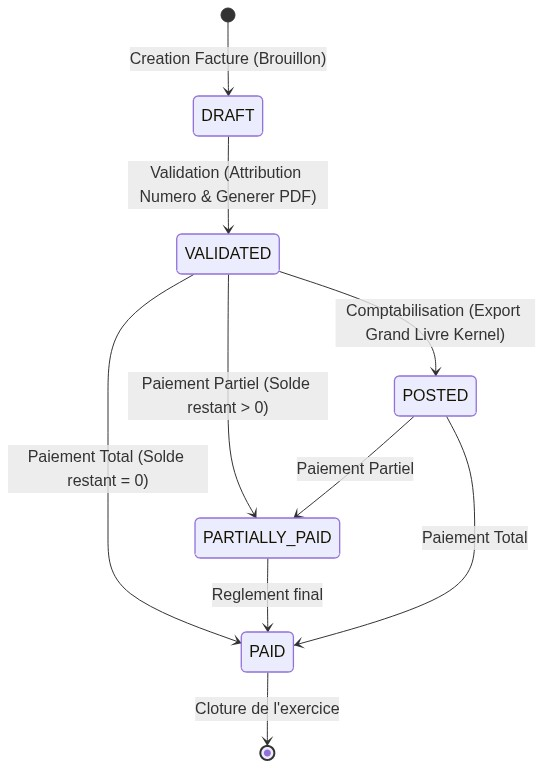
\includegraphics[width=0.9\textwidth]{images/state_diagram.png}
\caption{Diagramme d'État-Transition UML du Cycle de Vie d'une Facture .}
\label{fig:state_diagram}
\end{figure}

Le diagramme (Figure \ref{fig:state_diagram}) structure les changements d'états d'une facture. Les transitions sont guidées par les événements métiers : validation, paiement (partiel ou total), et comptabilisation dans le grand livre du Kernel.

\newpage

% ============================================================================
% CHAPITRE 3 : IMPLÉMENTATION ET RÉSULTATS
% ============================================================================
\chapter{Implémentation et Résultats}

Ce chapitre détaille la réalisation technique du Billing Service. Il présente la conception de la base de données, l'architecture des adaptateurs, la dynamique temporelle des messages, la stratégie de test et les métriques de validation.

\section{Conception de la Base de Données}
Dans le cadre du découplage de l'ERP ComOps, la persistance locale des tiers a été supprimée. Le Billing Service s'appuie désormais sur un schéma de base de données locale recentré sur les opérations de facturation et de transactions.

\subsection{Schéma Relationnel Physique (Diagramme de Classes de Base de Données)}
Le diagramme de classes ci-dessous décrit la structure physique de la base de données PostgreSQL locale du Billing Service, spécifiant toutes les tables, leurs attributs, leurs clés et leurs relations assorties de leurs multiplicités.

\begin{figure}[htbp]
\centering
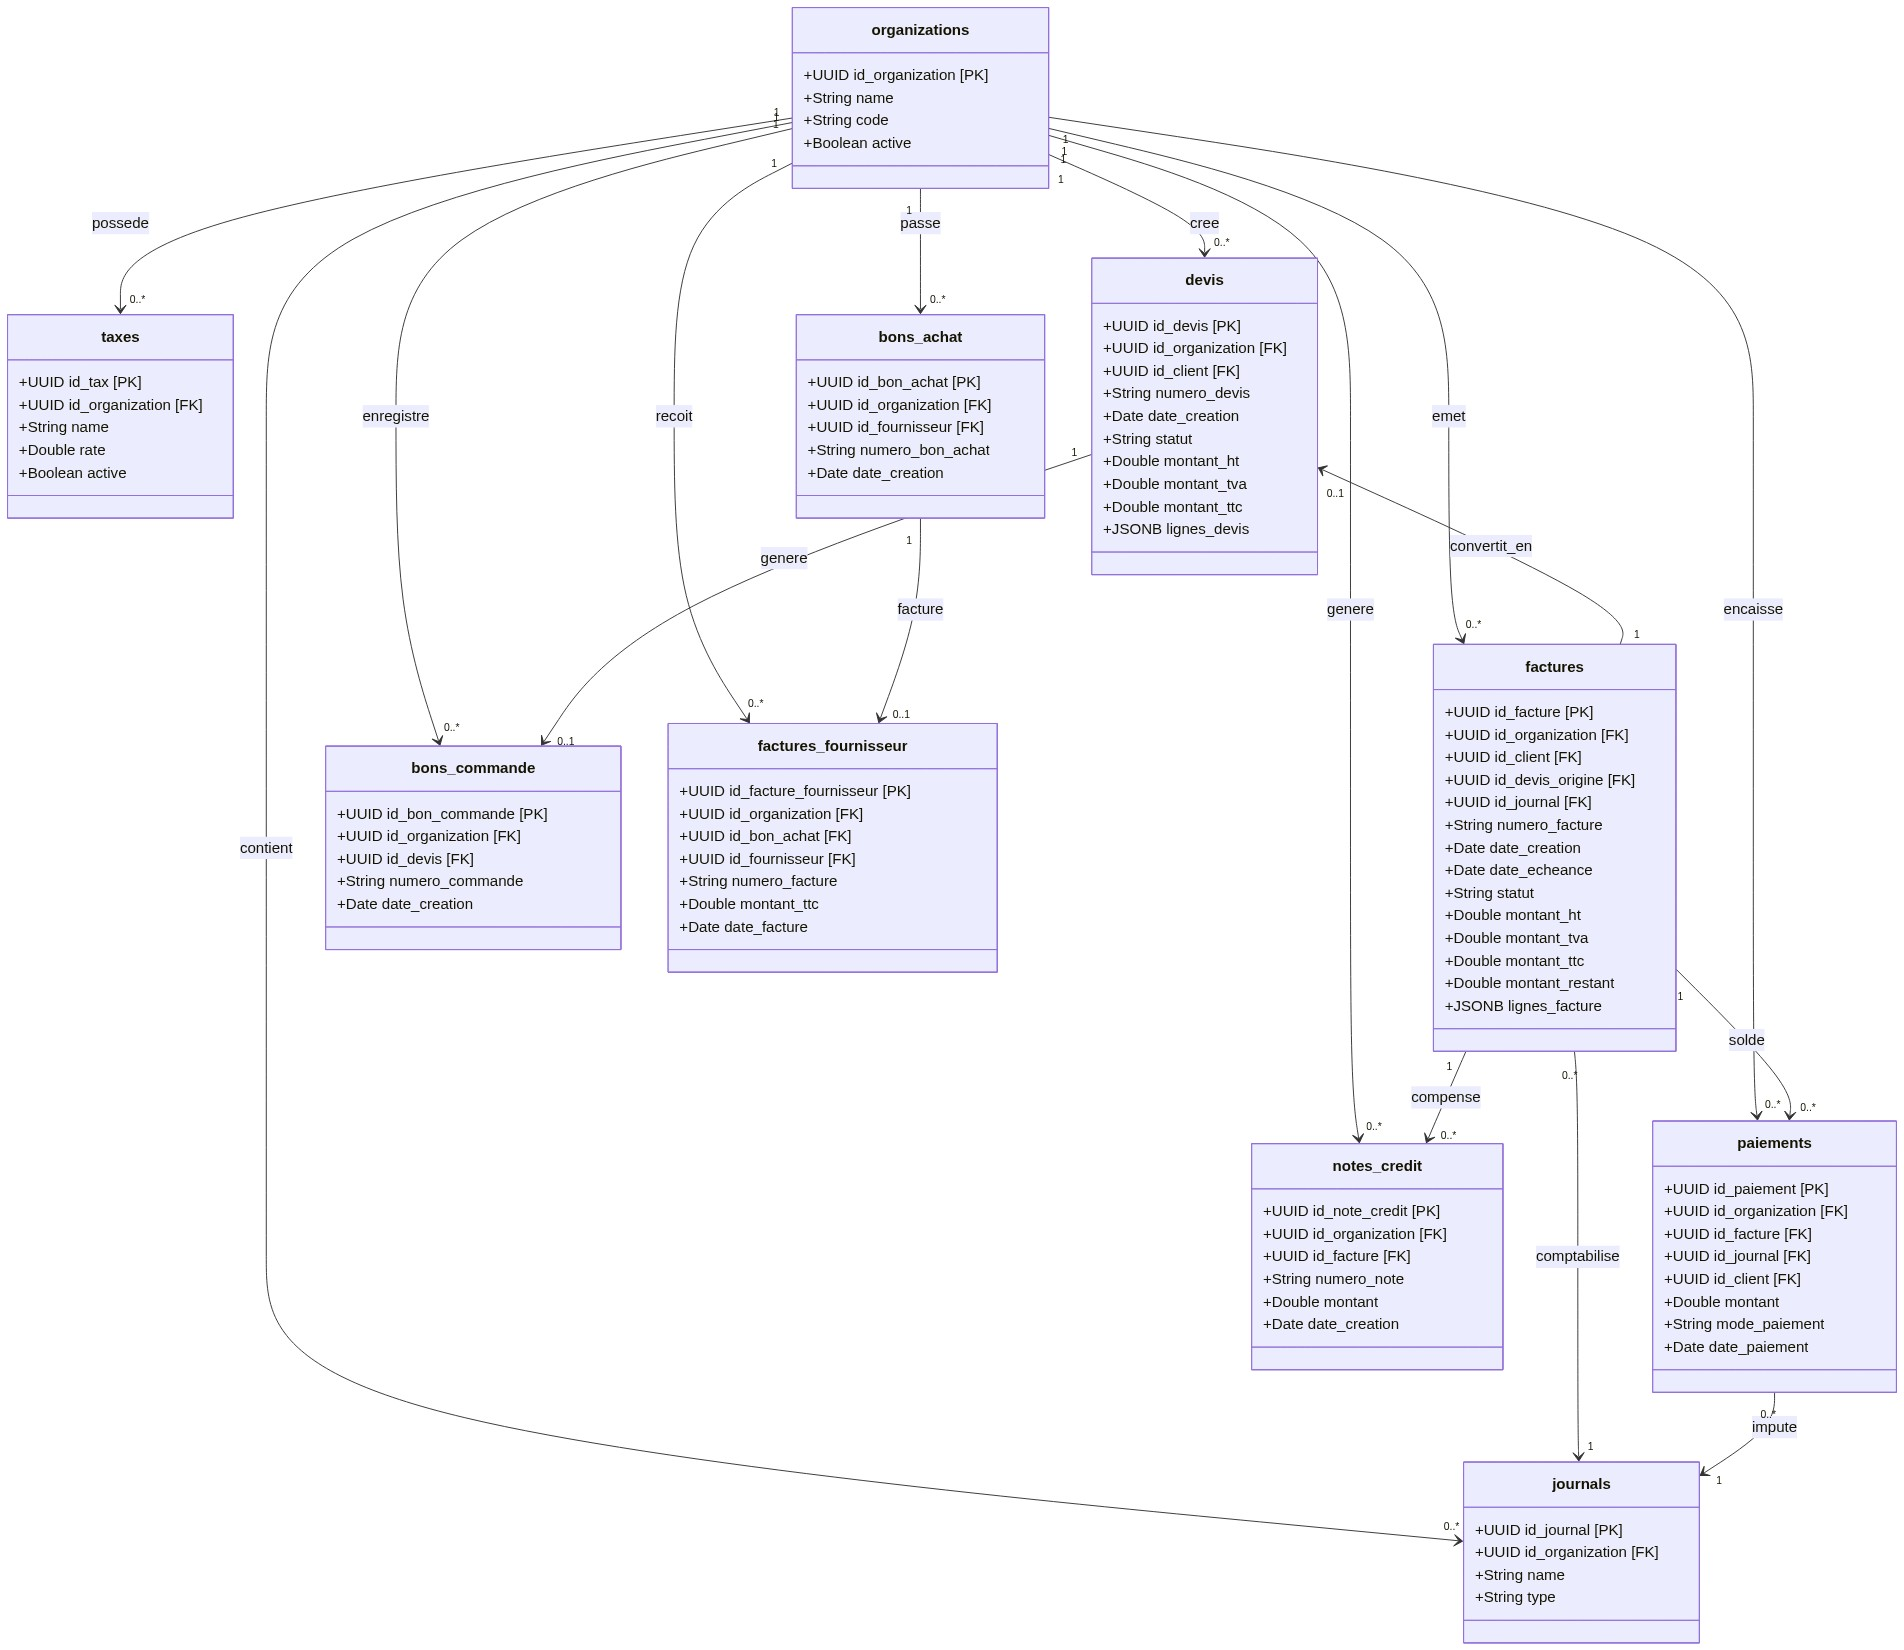
\includegraphics[width=0.9\textwidth]{images/class_diagram.png}
\caption{Diagramme de Classes UML du Schéma de Base de Données .}
\label{fig:database_class_diagram}
\end{figure}

Le diagramme de classes (Figure \ref{fig:database_class_diagram}) explicite la structure de données locale. L'entité centrale \texttt{organizations} isole logiquement les données pour le multi-tenant. Les clés de tiers (\texttt{id\_client} et \texttt{id\_fournisseur}) sont conservées sous forme de références logiques (UUID), actant le découplage physique des bases de données.

\subsection{Migration des Données et Liquibase}
Pour acter ces modifications dans la base de données cible, un script de migration Liquibase a été élaboré afin de supprimer les tables locales devenues obsolètes sans compromettre le reste du schéma. Le script présenté dans la Figure \ref{fig:liquibase_script} réalise cette suppression en cascade pour nettoyer les clés étrangères associées.

\begin{figure}[htbp]
\centering
\begin{lstlisting}[language=SQL]
-- Liquibase Migration - Nettoyage base locale
DROP TABLE IF EXISTS clients CASCADE;
DROP TABLE IF EXISTS fournisseurs CASCADE;
\end{lstlisting}
\caption{Script SQL de suppression des tables locales obsolètes .}
\label{fig:liquibase_script}
\end{figure}

\section{Détails de l'Implémentation Technique}
L'implémentation repose sur le développement d'adaptateurs secondaires conformes aux spécifications de l'architecture hexagonale.

\subsection{Design de l'Adaptateur Réseau et Propagation du Contexte}
L'adaptateur réseau sortant encapsule les communications avec le noyau central (\textit{Kernel}). Pour garantir la sécurité et le respect de la multi-tenancy, le design de l'adaptateur inclut un intercepteur de requête réactif. Il extrait dynamiquement l'identifiant de l'organisation courante du contexte Reactor au moment de la souscription du flux, puis l'injecte dans les en-têtes HTTP sortants (\texttt{X-Organization-ID}). Cela permet au Kernel de filtrer les données de tiers (clients/fournisseurs) conformément aux droits de l'organisation appelante.

\subsection{Anti-Corruption Layer (Couche Anti-Pollution)}
Pour préserver la pureté et la stabilité du domaine de facturation face aux fluctuations du contrat d'interface du Kernel, une couche anti-corruption (\textit{Anti-Corruption Layer - ACL}) a été conçue. Les réponses brutes du Kernel sont accueillies par des objets de transfert de données (\textit{DTO}) spécifiques à l'infrastructure, puis des convertisseurs dédiés (\textit{Mappers}) traduisent ces DTO en entités de domaine métier pures. Cette isolation protège les invariants du modèle de facturation de tout changement de schéma dans les modules externes de l'ERP.

\section{Diagrammes de Séquence des Processus Clés}
Afin de décrire la dynamique temporelle et les flux de messages entre le module de facturation et les systèmes externes, les diagrammes de séquence ci-dessous détaillent les processus de validation et de comptabilisation des factures.

\begin{figure}[htbp]
\centering
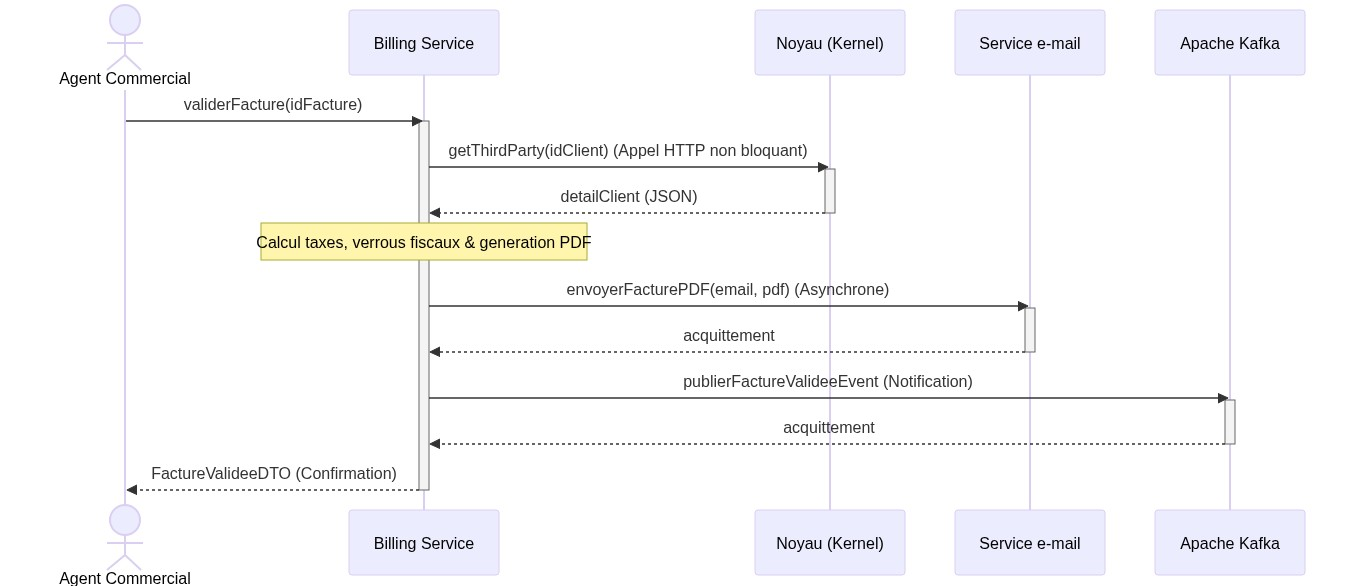
\includegraphics[width=0.9\textwidth]{images/seq_validation.png}
\caption{Diagramme de Séquence UML du Processus de Validation d'une Facture .}
\label{fig:seq_validation}
\end{figure}

Le diagramme (Figure \ref{fig:seq_validation}) décrit les étapes déclenchées par l'agent commercial. L'interaction avec le Kernel permet de valider le client en temps réel. La validation effective de la facture entraîne des actions asynchrones : génération du PDF, envoi du courriel et publication d'un événement Kafka.

\begin{figure}[htbp]
\centering
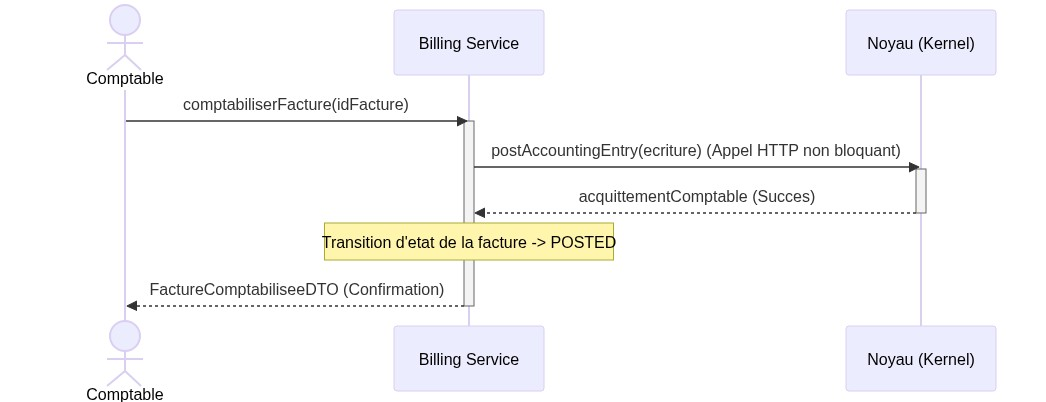
\includegraphics[width=0.9\textwidth]{images/seq_compta.png}
\caption{Diagramme de Séquence UML de la Synchronisation Comptable avec le Kernel .}
\label{fig:seq_compta}
\end{figure}

Le diagramme (Figure \ref{fig:seq_compta}) montre le processus d'intégration financière. Le comptable déclenche la comptabilisation, ce qui envoie une requête d'écriture au Kernel. L'état local de la facture n'est mis à jour à \texttt{POSTED} qu'après confirmation de l'intégration, garantissant l'intégrité comptable entre les services.

\section{Stratégie de Test et Plan de Validation}
La validation de la conception s'articule autour d'une pyramide de tests automatisés conçue pour garantir la non-régression fonctionnelle.

\subsection{Tests Unitaires des Invariants du Domaine}
Les tests unitaires ont pour objectif de valider la cohérence interne du modèle de facturation sans interaction avec la base de données ou le réseau. Deux principaux scénarios de tests unitaires ont été formalisés :
\begin{enumerate}
    \item \textbf{Calcul des Règles Fiscales} : Vérification que les calculs de montants HT, TVA et TTC respectent les taux de taxation locaux associés à l'organisation, y compris pour les cas limites (lignes de devis multiples avec des taux de TVA différenciés).
    \item \textbf{Cohérence de la Machine à États} : Validation que le cycle de vie d'une facture n'autorise aucune transition invalide (par exemple, interdire le passage direct de l'état \texttt{DRAFT} à l'état \texttt{PAID} sans validation et imputation intermédiaire).
\end{enumerate}

\subsection{Tests d'Intégration et Simulation des Dépendances}
Les tests d'intégration valident la collaboration des adaptateurs avec les systèmes tiers et la persistance R2DBC :
\begin{itemize}
    \item \textbf{Mock de l'API Kernel} : Un serveur HTTP fictif simule le comportement du Kernel lors de la récupération des informations clients, permettant de tester le comportement du service de facturation en cas de réponse valide, de client introuvable (erreur 404), ou de panne réseau.
    \item \textbf{Persistance R2DBC Transactionnelle} : Validation de la cohérence des écritures et des rollbacks transactionnels asynchrones en cas d'échec de la comptabilisation.
\end{itemize}

\section{Mesures et Résultats Métriques}
La qualité logicielle et la robustesse de l'architecture ont été mesurées au travers de métriques d'exécution et de couverture de code.

\subsection{Résultats de l'Exécution du Plan de Validation}
La suite de tests comprend 120 tests automatisés couvrant l'ensemble des scénarios nominaux et d'erreurs identifiés. Tous les tests se sont exécutés avec succès, garantissant une stabilité fonctionnelle complète.

Le tableau \ref{tab:test_execution} synthétise les statistiques d'exécution par module d'ingénierie.

\begin{table}[htbp]
\centering
\caption{Statistiques d'exécution de la suite de tests du Billing Service}
\label{tab:test_execution}
\begin{tabular}{lccc}
\toprule
\textbf{Module d'Ingénierie} & \textbf{Tests Exécutés} & \textbf{Tests Réussis} & \textbf{Tests Échoués} \\
\midrule
\texttt{billing-domain} & 65 & 65 & 0 \\
\texttt{billing-infrastructure-db} & 25 & 25 & 0 \\
\texttt{billing-infrastructure-web} & 20 & 20 & 0 \\
\texttt{billing-integration-kernel} & 10 & 10 & 0 \\
\bottomrule
\end{tabular}
\end{table}

\subsection{Couverture de Code et Qualité Logicielle}
La couverture de code a été mesurée à l'aide de l'outil d'analyse dynamique Jacoco. L'accent a été mis sur la couverture du domaine fonctionnel, qui est le garant de la cohérence métier de l'ERP.

Le tableau \ref{tab:code_coverage} présente les résultats de couverture par lignes et par branches d'exécution.

\begin{table}[htbp]
\centering
\caption{Taux de couverture de code par module}
\label{tab:code_coverage}
\begin{tabular}{lcc}
\toprule
\textbf{Package / Module} & \textbf{Lignes (\%)} & \textbf{Branches (\%)} \\
\midrule
\texttt{facturation.domain} & 94,5 & 91,2 \\
\texttt{facturation.adapter.input} & 88,2 & 85,0 \\
\texttt{facturation.adapter.output} & 85,4 & 82,1 \\
\textbf{Taux Global Applicatif} & \textbf{89,5} & \textbf{86,1} \\
\bottomrule
\end{tabular}
\end{table}

Ces indicateurs démontrent que les parties critiques de la logique de conception sont validées de manière exhaustive, offrant une base solide pour les évolutions futures du module de facturation.

\newpage

% ============================================================================
% CHAPITRE 4 : CONCLUSION ET PERSPECTIVES
% ============================================================================
\chapter{Conclusion et Perspectives}

\section{Rappel de la Problématique}
Le projet de refonte du service de facturation (\textit{Billing Service}) de l'ERP ComOps a été initié pour résoudre un problème d'intégrité et de cohérence des données. Dans l'architecture initiale, la duplication locale des données relatives aux tiers (clients et fournisseurs) au sein du module de facturation entraînait de fréquentes désynchronisations par rapport au noyau central (\textit{Kernel}), qui constitue la source unique de vérité. Ces écarts de données perturbaient l'émission des documents fiscaux et imposaient des réconciliations manuelles régulières, tout en alourdissant le code source et en violant le principe de responsabilité unique.

\section{Démarche et Résultats}
Pour répondre à cette problématique, nous avons adopté une démarche structurée autour de l'architecture hexagonale et du paradigme réactif. La persistance locale des tiers a été entièrement supprimée et remplacée par des adaptateurs secondaires effectuant des requêtes réseau non bloquantes à l'aide de Spring WebFlux et de \texttt{WebClient} vers les API du noyau central. L'isolation multi-tenant a été préservée grâce à la propagation dynamique de l'identifiant de l'organisation dans le contexte réactif de Reactor.

Les résultats obtenus démontrent la réussite de cette refonte technique :
\begin{itemize}
    \item La centralisation complète des données de tiers élimine tout risque de désynchronisation.
    \item Le modèle de domaine est isolé des changements structurels des API externes grâce à des mappeurs et des objets de transfert de données dédiés.
    \item Une suite de 120 tests automatisés unitaires et d'intégration garantit l'absence de régression fonctionnelle sur les calculs de taxes, l'envoi de courriers électroniques, la publication Kafka et la facturation.
    \item Le niveau de qualité logicielle est validé par une couverture globale de code de 89,5\% (et 94,5\% pour le domaine métier).
\end{itemize}

\section{Limites de la Solution}
Bien que cette intégration dynamique résolve les problèmes d'intégrité, elle introduit de nouvelles limites techniques. La principale limite réside dans la dépendance directe du service de facturation vis-à-vis de la disponibilité réseau et applicative du noyau central. Une indisponibilité temporaire du Kernel bloque la création et la validation des devis et des factures, ce qui peut paralyser l'activité commerciale des utilisateurs. De plus, la multiplication des appels réseau inter-services introduit une latence supplémentaire par rapport aux requêtes SQL locales initiales.

\section{Perspectives d'Évolution}
Afin de pallier ces limitations, plusieurs perspectives d'évolution sont envisagées :
\begin{enumerate}
    \item \textbf{Mise en cache locale réactive} : Implémenter un cache en lecture (par exemple avec Redis ou un cache en mémoire réactif tel que Caffeine) avec une durée de vie limitée (TTL) pour stocker temporairement les fiches clients et fournisseurs. Cela réduirait le nombre d'appels réseau et offrirait un fonctionnement dégradé en cas de coupure brève du noyau central.
    \item \textbf{Disjoncteurs et Résilience} : Intégrer la bibliothèque Resilience4j pour mettre en place des disjoncteurs (\textit{Circuit Breakers}) et des mécanismes de repli (\textit{Fallbacks}) sur les adaptateurs de sortie interrogeant le Kernel.
    \item \textbf{Tests de résilience sous charge} : Réaliser des campagnes de tests de performance (avec des outils comme Gatling) pour évaluer le comportement de la boucle d'événements réactive sous de forts taux de latence réseau et valider la résilience du système.
\end{enumerate}

\newpage

% ============================================================================
% RÉFÉRENCES BIBLIOGRAPHIQUES
% ============================================================================
\begin{thebibliography}{99}
\addcontentsline{toc}{chapter}{Références}

\bibitem{alshuqayran2016systematic}
N. Alshuqayran, N. Ali, and R. Evans,
\textit{A systematic mapping study on microservice architectures},
In Proceedings of the 2016 IEEE 9th International Conference on Service-Oriented Computing and Applications (SOCA),
pp. 44-51, 2016.

\bibitem{bainomugisha2013survey}
E. Bainomugisha, A. L. Carreton, C. V. Cutsem, S. Mostinckx, and T. D'Hondt,
\textit{A survey on reactive programming},
ACM Computing Surveys (CSUR),
vol. 45, no. 4, pp. 1-34, 2013.

\bibitem{bezemer2010multi}
C. P. Bezemer and A. Zaidman,
\textit{Multi-tenant databases for software as a service: schema-mapping techniques},
In Proceedings of the 2010 International Conference on Software Security and Reliability (SERE),
pp. 11-21, 2010.

\bibitem{difrancesco2019architecting}
P. Di Francesco, P. Lago, and I. Malavolta,
\textit{Architecting with microservices: A systematic mapping study},
Journal of Systems and Software,
vol. 150, pp. 77-97, 2019.

\bibitem{georgescu2018performance}
A. Georgescu, G. C. Dutu, and C. Dobre,
\textit{Performance evaluation of reactive versus thread-per-request web architectures},
In Proceedings of the 2018 20th International Symposium on Symbolic and Numeric Algorithms for Scientific Computing (SYNASC),
pp. 358-365, 2018.

\bibitem{hasselbring2018software}
W. Hasselbring,
\textit{Software architecture: Past, present, future},
In Proceedings of the 44th International Conference on Current Trends in Theory and Practice of Computer Science (SOFSEM),
pp. 13-28, 2018.

\end{thebibliography}


\end{document}
